
%%%
% Any line that begins with a percent symbol is a comment. To compile
% this document and view the output:
%
% Run Latex
% Run Bibtex
% Then run Latex twice.
%
% This should produce the output PDF file named main.pdf
%%%

% This defines the style to use for this document.
% Do not modify.
\documentclass[letterpaper]{article}

% The following are akin to "import" statements in Python or Java -
% these import useful commands into the document for you to use.  You
% don't have to modify any of these lines. The AAAI package formats
% this document in the style of submissions to the American
% Association for Artificial Intelligence conference, one of the top
% AI conferences in the world. You will find that many academic
% publications in AI use this format.
\usepackage{aaai} 
\usepackage{times} 
\usepackage{helvet} 
\usepackage{courier} 
\setlength{\pdfpagewidth}{8.5in} 
\setlength{\pdfpageheight}{11in} 
\usepackage{amsmath}
\usepackage{amsthm}
\usepackage{graphicx}
\usepackage{graphics}
\usepackage{moreverb}
\usepackage{subfigure}
\usepackage{epsfig}
\usepackage{txfonts}
\usepackage{algpseudocode}
\usepackage{multirow, multicol}
\usepackage{url}
\usepackage{tablefootnote}
\usepackage{color}
\usepackage{pgfplots}

\setcounter{secnumdepth}{1}
\nocopyright

% Fill in your paper title, names and emails below
% The "\\" is used to break lines. The \url command
% is useful for typesetting URLs and email addresses (it uses the
% Courier font).
\title{Genetic Programming and Fantasy Baseball}
 \author{Alexander Donald \and Gabriel Levy\\
 \url{{aldonald, galevy}@davidson.edu}\\
 Davidson College\\
 Davidson, NC 28035\\
 U.S.A.}

% This is the "true" start of the document. All the text in your
% write-up should be placed within the \begin{document} and
% \end{document} decorators.
\begin{document}

\maketitle % formats the title nicely, do not modify

% While at this point you could just begin your write-up, often, it's
% useful to write each section of your write-up in a separate tex
% file (not unlike the modular decomposition you do for code you
% write). These \input commands insert the contents of the
% specified tex files in the order specified. Every write-up you
% submit must contain the following sections, in the shown order. Open
% each of the indicated tex files to understand what goes in each
% section, as well as for more TeX tips.

% Place the contents of your abstract between the
% \begin{abstract} and \end{abstract} decorators.

\begin{abstract}
In this study, we explored existing methods of genetic programming and modified them to best build fantasy lineups for Major League Baseball. Specifically, we were interested in maximizing a team's point total given a budget. We utilize variations of genetic programming techniques to analyze teams and players given their fantasy preseason option value and 2021 season statistics to build the optimal team by smartly allocating a given budget.


% The \textbf{} command makes the specified text bold. The \emph{} or
% \textit{} command are used to italicize text. In general, text is never
% underlined.

% DON'T FORGET TO MATCH EACH OPEN BRACE WITH A CLOSING BRACE!
\end{abstract}



% The \section{} command formats and sets the title of this
% section. We'll deal with labels later.
\section{Introduction}
\label{sec:intro}

DraftKing.py is our final genetic program that uses an analysis of prices and fantasy points of Major League Baseball players to evolve the best possible fantasy baseball lineup given a specified budget. A budget restricts fantasy players from picking all the best MLB players with the most points, meaning you must find players with low prices but solid points to complement higher cost players. DraftKing takes into account both point contribution and price of players when determining fitness of teams and how to evolve them. 

We used two datasets when testing DraftKing. The first data set from Sporting News holds 2021 MLB player pre-season auction prices \cite{optionPrice}. This data is used when calculating the cost of a team. The second data set from Baseball Savant contains 2021 season statistics for both hitters and pitchers used in calculating a player's fantasy points \cite{stats}. \\

This paper is organized as follows. Our background section discusses the formula used to calculate fantasy points and some information about how DraftKing evolves generations of individuals, specifically through crossover and mutation. The experiments section describes the process of developing, fine tuning, and testing DraftKing in order to build the best lineups in an efficient manner. We will include a comparison of two slightly different variations. In the results section, we analyze the output of DraftKing at peak performance. We will look at the quality of the final lineups produced and analyze the frequency that certain players showed up. Our conclusion summarizes our findings.

% Citations: As you can see above, you create a citation by using the
% \cite{} command. Inside the braces, you provide a "key" that is
% uniue to the paper/book/resource you are citing. How do you
% associate a key with a specific paper? You do so in a separate bib
% file --- for this document, the bib file is called
% project1.bib. Open that file to continue reading...

% Note that merely hitting the "return" key will not start a new line
% in LaTeX. To break a line, you need to end it with \\. To begin a 
% new paragraph, end a line with \\, leave a blank
% line, and then start the next line (like in this example).
%Overall, the aim in this section is context-setting: what is the
% big-picture surrounding the problem you are tackling here?





\section{Background}
\label{sec:background}

\subsection{Data Preparation}
\label{subsec:enum}
In order to get total points for each MLB player, we used a formula that took in our 2021 season stats data combined with a fantasy points scoring system from fantasydata.com and spit out a points value \cite{pointsSystem}. For example, if a hitter had 21 doubles during the season, that would correlate to $2(21) = 42$ fantasy points since 1 double counts as 2 points. The formula for hitters is as follows \footnote{\url{https://baseballxgear.com/baseball-stats-abbreviations-what-do-they-mean}}
$$4(\text{HR}) + 3(\text{3B}) + 2(\text{2B} + \text{RBI} + \text{SB}) + \text{1B} + \text{R} + \text{BB} + \text{HBP}  - \text{CS} - .5(\text{SO})$$
The formula for pitchers is as follows:
$$5(\text{W}) + 3(\text{S}) + \text{IP} + \text{SO} - 3(\text{BS}) -  2(\text{ER}) - \text{BB} -  \text{HBP} - .5(\text{H})$$

These formulas allowed us to score players based on their statistics using a standardized fantasy baseball scoring system. 


\subsection{Lineups}
\label{subsec:enum}
Our fantasy lineups consist of 1 catcher, 1 first basemen, 1 second basemen, 1 third basemen, 1 shortstop, 1 designated hitter, 3 outfielders, 5 starting pitchers, and 5 relief pitchers for a total of 19 players. In our genetic program, we model these lineups with an array that has indices corresponding to specific positions. 

\subsection{Budget}
\label{subsec:enum}
For DraftKing, the budget was set at \$200. This means that the sum of the costs of every player in a team's lineup must be less than this budget. We felt that \$200 gave us enough room to build a very solid team, but not enough cash to make a team of all the most highly regarded and pricey MLB players. 

\subsection{Genetic Programming Techniques}
\label{subsec:enum}
To decide what lineups are best within each generation, DraftKing uses the total fantasy points of all players on a team as the fitness function. Although this function does not take into account the cost of players, the budget constraint and genetic programming operations lead to adequate cost control so that a balanced team is built. DraftKing uses three main genetic programming strategies which are crossover, selective mutation, and reproduction. We will now provide the reader with a brief overview of these strategies including a description of regular mutation:
\begin{itemize}
	\item Crossover takes 2 lineups and creates 2 new lineups by crossing over the initial lineups at a somewhat random crossover point. By somewhat, we mean our crossover point chooses randomly except at positions where there are multiple players (outfield, starting pitcher, relief pitcher). In the case that there are multiple players at a position, we crossover at the first instance of that position in our lineup to avoid repetition of players due to crossover. 
    \item Mutation takes 1 lineup and returns 1 lineup with 1 modified player. An index within the lineup is chosen at random and that player is replaced with a random player of the same position.
	\item Selective Mutation takes 1 lineup and returns 1 lineup with 1 modified player. A mutation index within the lineup is chosen selectively based on a metric. When a team's cost is within $90\%$ of the budget this metric is the percentage of fantasy points contributed by this player to the whole team minus the percentage of the team's budget taken up by the player. When a team's cost is below $90\%$ of the budget, this metric is the player with the lowest fantasy point contribution. Once the mutation index is chosen, the player at that index is replaced with a more optimal player. In the first case mentioned above this a player with a higher difference between percent of points and percent of budget than the old player. In the second case this is a player with more overall fantasy points. 
	\item Reproduction reproduces the top lineups of each generation in order to make sure the most fit individuals persist through generations.
\end{itemize}

In the experiments section of our paper, we will examine in depth the advantages of using selective mutation and the parameters of our genetic program as a whole that contributed to its success. 







\section{Experiments}
\label{sec:expts}

\subsection{Parameters}
\label{subsec:enum}
Some of the key parameters that we had to decide on for our genetic program were generation size, number of generations, and the percentage of individuals to perform each of our genetic operations on. For generation size, we stuck with 50 individuals because of the diversity and speed that it provided. In general, lower generation sizes yielded less diversity leading to lower plateaus of the best team's score while significantly higher generation sizes lead to significantly slower run time. For number of generations, we played around with this depending on what we were testing, however, 250 generations seems to give a good idea of what the final team will look like. This number might change depending on some of the variations of the genetic operations we implement. We will discuss the effects of number of generations later in this section. Concerning genetic operations, the breakdown of DraftKing's percentages are the following: crossover on $80\%$ of individuals, mutation on $15\%$ of individuals, and regeneration of $5\%$ of individuals. We decided on these percentages because they gave DraftKing the ability to make significant improvements with crossovers, yet mutate a decent number of individuals in attempt to fine-tune the lineups. Mutation was especially important given that crossover indices were selected to make sure groups of players in the same position were not broken up to avoid duplicate players. Therefore, if the first starting pitcher was selected as the crossover point, all the starting pitchers would be crossed over. Mutation would then allow this group of starting pitchers to be modified. Regenerating $5\%$ of individuals made sure that some of the most fit individuals will be carried onto the next generation, keeping their quality traits in the gene pool. 


\subsection{Implementing Selective Mutation}
\label{subsec:enum}
During initial experimentation, we used basic crossover, mutation, and reproduction as described in the Background section. We were able to get solid lineups, however, it took hundreds of generations to reach them. We decided to create a selective mutation operation that mutated weak parts of a team. Initially, we created a selective mutation method that chose a mutation index based off the player with the worst value on the team determined by the equation $points_x \div points_{team} - cost_x \div cost_{team}$ where $x$ is the current player and $team$ is the entire team. Once this player was selected, they were randomly replaced with another player. However, we realized that this player was often replaced with a player with fewer points. Even though they were a better value based on our equation, they did not help maximize the team's score. This method of mutation did not account for the fact that we had a budget that could be used fully without consequence. This method would be much more useful to maximize a lineup at minimum cost. Therefore we implemented a cutoff at $90\%$ of the total budget. Any team with less than this cutoff value would be mutated using a different metric. This metric was a player's points. The mutation index for all teams with a cost less that this cutoff value would be that of the player with the least amount of points. The combination of these two metrics was extremely effective. The program now was able to realize that it could splurge on expensive players when the budget was there, significantly increasing the point total. We were also then able to find more optimal lineups when the budget got tight, replacing overvalued players with more successful cost-efficient players. We will now compare this mutation method to regular random mutation.


\subsection{Regular Mutation vs. Selective Mutation}
\label{subsec:enum}
Our main experiment consisted of testing regular random mutation vs. selective mutation, seeing how total points varied between genetic programs using the two methods after a certain amount of generations. All runs were completed with a generation size of 50 individuals and crossover, mutation, and reproduction ratios of $0.8$, $0.15$, and $0.05$. The results are seen in Figure 1.



\begin{figure}
\centering
    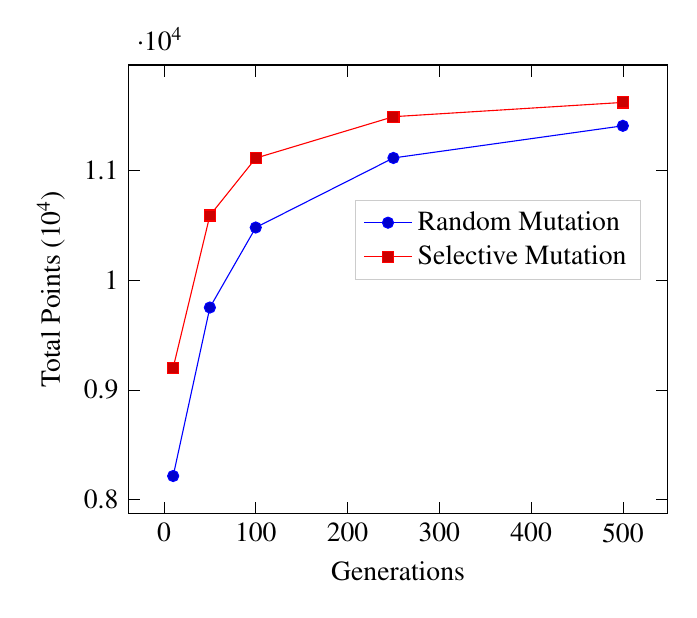
\begin{tikzpicture}
      \begin{axis}[
        legend cell align={left},
        legend style={draw=white!80.0!black, at={(.95,.7)},anchor= north east},
        x grid style={white!69.01960784313725!black},
        xlabel={Generations},
        xtick style={color=black},
        y grid style={white!69.01960784313725!black},
        ylabel={Total Points ($10^4$)},
        ytick style={color=black}
        ]
        \addplot coordinates {
          (10,  8214.6)
          (50,  9751.2)
          (100,  10481.0)
          (250, 11115.5)
          (500, 11408.6)
        };
        \addlegendentry{Random Mutation}
        \addplot coordinates {
          (10,  9201.5)
          (50,  10590.8)
          (100,  11113.9)
          (250, 11491.9)
          (500, 11622.1)
        };
        \addlegendentry{Selective Mutation}
      \end{axis}
    \end{tikzpicture}
\caption{Plot showing the progression of average total team scores of genetic programs with selective mutation versus those with random mutation. Each point represents the average team points total for 10 runs at a given generation size.}
\end{figure}





Based on this experiment, it is clear that the selective mutation is more effective at building better teams quicker. This makes sense given that when selective mutation is used, a team's weakness is most definitely improved upon mutation, while random mutation could easily make the player at a given position worse. This experiment also gives us an idea of the number of generations needed to find the optimal team. Based off the averages and Figure 1, it is clear that teams are still improving up until 500 generations in both cases. We believe that after 500 generations, a team is very near, if not at, the peak of where it can get. Especially when using selective mutation, we saw little to no improvement once generations got near 500, as seen in the plateauing of selective mutation in Figure 1. Runs using regular mutation might still see a bit of improvement after 500 given that these teams tend to plateau after higher numbers of generations. Overall, Figure 1 demonstrates that selective mutation significantly increases the effectiveness and speed of our genetic program.


\section{Results}
\label{sec:results}

We ran our final program, DraftKing, with selective mutation, a generation size of 50, 500 generations, a budget of \$200, and crossover, mutation, and reproduction ratios of $0.8$, $0.15$, and $0.05$. We conducted $20$ trials with these parameters, which resulted in the following highest-scoring lineup found here in Figure 2.

\begin{figure}[htb]
  \centering 
  \begin{tabular}{|c|c|c|c|} 
    \hline \hline 
    Position & Player & Price & Points \\ 
    \hline 
    Catcher & Salvador Perez & $14$ & $625$ \\
    First Base & Matt Olson & $15$ & $675.5$ \\
    Second Base & Max Muncy & $10$ & $582$ \\
    Third Base & Vladimir Guerrero Jr. & $20$ & $752$ \\
    Shortstop & Jorge Polanco & $3$ & $596$ \\
    Outfield & Bryan Reynolds & $3$ & $596.5$ \\
    Outfield & Mitch Haniger & $4$ & $591.5$ \\
    Outfield & Austin Riley & $5$ & $597$ \\
    DH & Marcus Semien & $12$ & $697$ \\
    Starter & Robbie Ray & $2$ & $632.75$ \\
    Starter & Walker Buehler & $27$ & $631.75$ \\
    Starter & Max Scherzer & $28$ & $716.5$ \\
    Starter & Zack Wheeler & $9$ & $649$ \\
    Starter & Julio Urias & $4$ & $594.25$ \\
    Reliever & Corbin Burnes & $8$ & $661.25$ \\
    Reliever & Freddy Peralta & $2$ & $475.25$ \\
    Reliever & Liam Hendricks & $14$ & $583.75$ \\
    Reliever & Raisel Iglesias & $9$ & $502.5$ \\
    Reliever & Kevin Gausman & $6$ & $600$ \\
    \hline 
    Total & & $195$ & $11759.5$ \\
    \hline \hline
  \end{tabular}

  \caption{Highest-scoring lineup found in 20 trials.}
  \label{tab:example}

\end{figure}

This lineup had the best score that we found in our $20$ trials. With a price of \$195, we cannot say for certain the lineup could not do better, however, it definitely limits how much better this lineup could become. 
\newline\indent The maximum price and points for all available hitters and pitchers respectively were $\$60$, $\$48$, $752$, and $716.5$. The average price and average points totaled by all hitters available to the program were $\$11.85$ and $417.62$ respectively. The hitters in this lineup had averages of $\$9.56$ and $634.72$. All pitchers carried averages of $\$7.64$ and $567.82$, while the pitchers in this lineup cost $\$10.9$ and produced $604.7$. From this data, it seems the hitters were selected more efficiently than the pitchers, led by Vladimir Guerrero who contributed more points than any hitter available in the simulation. The pitchers had the two highest-priced players on the team in Max Scherzer and Walker Buehler. However, Max Scherzer produced more points than any pitcher in the entire program, and Walker Buehler was nearly the third highest-producing pitcher on the team. So while a lot of money was spent on these two, the team may have needed their points. 
\newline\indent This is only one lineup that was created out of the $20$ trials that we ran with the program. Other lineups contained some of the same players and some different ones. Within the $20$ trials, we found the following pitchers and hitters $15$ or more times.


\begin{figure}[htb]
  \centering 
  \begin{tabular}{|c|c|c|c|} 
    \hline \hline 
    Player & Price & Points & Frequency \\ 
    \hline 
    Julio Urias & $4$ & $594.25$ & $20$ \\
    Kevin Gausman & $6$ & $600$ & 
    $20$ \\
    Corbin Burnes & $8$ & $661.25$ & $20$ \\
    Liam Hendricks & $14$ & $583.75$ & $19$ \\
    Robbie Ray & $2$ & $632.75$ & $19$ \\
    Raisel Iglesias & $9$ & $502.5$ & $18$ \\
    Max Scherzer & $28$ & $716.5$ & $18$ \\
    Zack Wheeler & $9$ & $649$ & $18$ \\
    Freddy Peralta & $2$ & $475.25$ & $15$ \\
    \hline 
    Average & & $9.11$ & $601.69$ \\
    \hline \hline
  \end{tabular}

  \caption{Most occurring pitchers.}
  \label{tab:example}

\end{figure}

\begin{figure}[htb]
  \centering 
  \begin{tabular}{|c|c|c|c|} 
    \hline \hline 
    Player & Price & Points & Frequency \\ 
    \hline 
    Salvador Perez & $14$ & $625$ & $20$ \\
    Bryan Reynolds & $3$ & $596.5$ & 
    $20$ \\
    Ausitn Riley & $5$ & $597$ & $20$ \\
    Vladimir Guerrero Jr. & $19$ & $752$ & $17$ \\
    Marcus Semien & $12$ & $697$ & $17$ \\
    \hline 
    Average & & $10.8$ & $653.5$ \\
    \hline \hline
  \end{tabular}

  \caption{Most occurring hitters.}
  \label{tab:example}

\end{figure}

It is obvious why some players showed up so many times. Robbie Ray only costs $\$2$, but he produced $632.75$ points. In 2021, he won the American League Cy Young Award for best pitcher in the American League. Vladimir Guerrero Jr. had an enormous $752$ points. While $\$19$ is a slightly higher price, he was the highest scoring hitter available. Other players can confuse people on why they may have been chosen so often. One player might be Raisel Iglesias. With a price equal to that of Zack Wheeler who produced $649$ points, Raisel Iglesias carried less points than anyone else on this list other than the extremely low-priced Freddy Peralta. But while it seems like Iglesias might not have as much value, no player that wasn't already on the best lineup could have replaced Iglesias and added more points while staying under the budget. In fact, the only reliever not on the roster who had more points was Josh Hader, who had $520.5$ points, but a price of $\$15$, good for the most expensive relief pitcher available. Hader found his way into $11$ out of the $20$ lineups. Concluding the results, this lineup produced was very good, and while it could likely be slightly improved, the genetic program seems to have done a great job finding an optimal lineup out of the players available within a budget constraint.





\section{Conclusions}
\label{sec:concl}

In this paper, we set out to find an optimal fantasy baseball lineup given players with auction prices and points produced and being constrained to budget. DraftKing found an incredible lineup that included well above average points for both hitters and pitchers. The number of generations was capped at $500$, which means that a slightly better lineup could have been accomplished given more time. The “optimal" lineup we found was a lineup found in hindsight. With the prices being from before the 2021 season and the points based off of 2021 stats, people actually drafting these players at these prices would not have the information we were given. Additionally, this is an optimal lineup if a manager of a fantasy baseball team was required to keep all of the players for the entire season. In reality, many leagues allow managers to trade, release, and add players throughout the season. This means that players who had incredible first parts of the season but then got injured might not be included in lineups, but would definitely be owned by real fantasy baseball managers. With all of this in mind, an interesting extension would be to look at the optimal lineup as the season progressed, allowing for changes in the roster. However, this would need stats from every player for every day of the $162$ game season, which unfortunately might not be entirely feasible. Given the stats and prices available to us, we believe we can and did find value in players that was not expected heading into the season and showed some players that exceeded all expectations.

\section{Contributions}
\label{sec:contrib}

A.D and G.L collectively wrote the program and ran experiments. A.D wrote the Introduction, Background, and Experiments sections. G.L wrote the Results and Conclusion sections.



% This creates the references section. Open the project1.bib file to
% see how to organize your references.
\bibliography{project1}
\bibliographystyle{aaai} % sets citation and bib style, do not modify



\end{document}
